
%Superscripts and subscripts that are words or abbreviations, as in
%\( \pi_{\mathrm{low}} \), should be typed as roman letters; this is
%done as \verb|\( \pi_{\mathrm{low}} \)| instead of \( \pi_{low} \)
%done by \verb|\( \pi_{low} \)|.

%User-defined macros should be placed in the preamble of the chapter,
%and not at any other place in the document. Definitions made using
%the commands \verb|\newcommand,| \verb|\renewcommand,|
%\verb|\newenvironment| or \verb|\renewenvironment| should be used
\newcommand{\Br}{\ensuremath{B\!\rho}}
\newcommand{\bull}{\ensuremath{\bullet~}}
\newcommand{\Bz}{\ensuremath{{B_z}}}
\newcommand{\com}{\ensuremath{\it com}}
\newcommand{\dip}{{\it DIPOLE}}
\newcommand{\EFB}{\ensuremath{E\!F\!B}}
\newcommand{\EFBs}{\ensuremath{E\!F\!B\!s}}
\newcommand{\ffag}{{\it FFAG}}
\newcommand{\lab}{\ensuremath{lab}}
\newcommand{\MC}{Monte~Carlo}


\chapter[Cyclotron]{Cyclotron}\label{chapCyclotron}


\section{Introduction}\label{secCycloIntro}

%You can obtain these files from our web pages at:
%\url{http://www.worldscientific.com/page/authors/book-stylefiles} and
%\url{http://www.icpress.co.uk/authors/stylefiles.shtml#books}.

Beyond simple knowledge and concepts, this Chapter introduces to the basic principles and formulas attached 
to the cyclotron, 
which will be manipulated during the user computer exercises. 
Deeper insight in the theory and technology 
of the cyclotron 
can be found in the brief series of refrences cited in this chapter. 
The candidate to the computer exercises which follow is encouraged to first read these references. 


\section{Cyclotron \label{secCyclotron}}

\begin{figure}[ht]
\centering
\sidebyside
{
    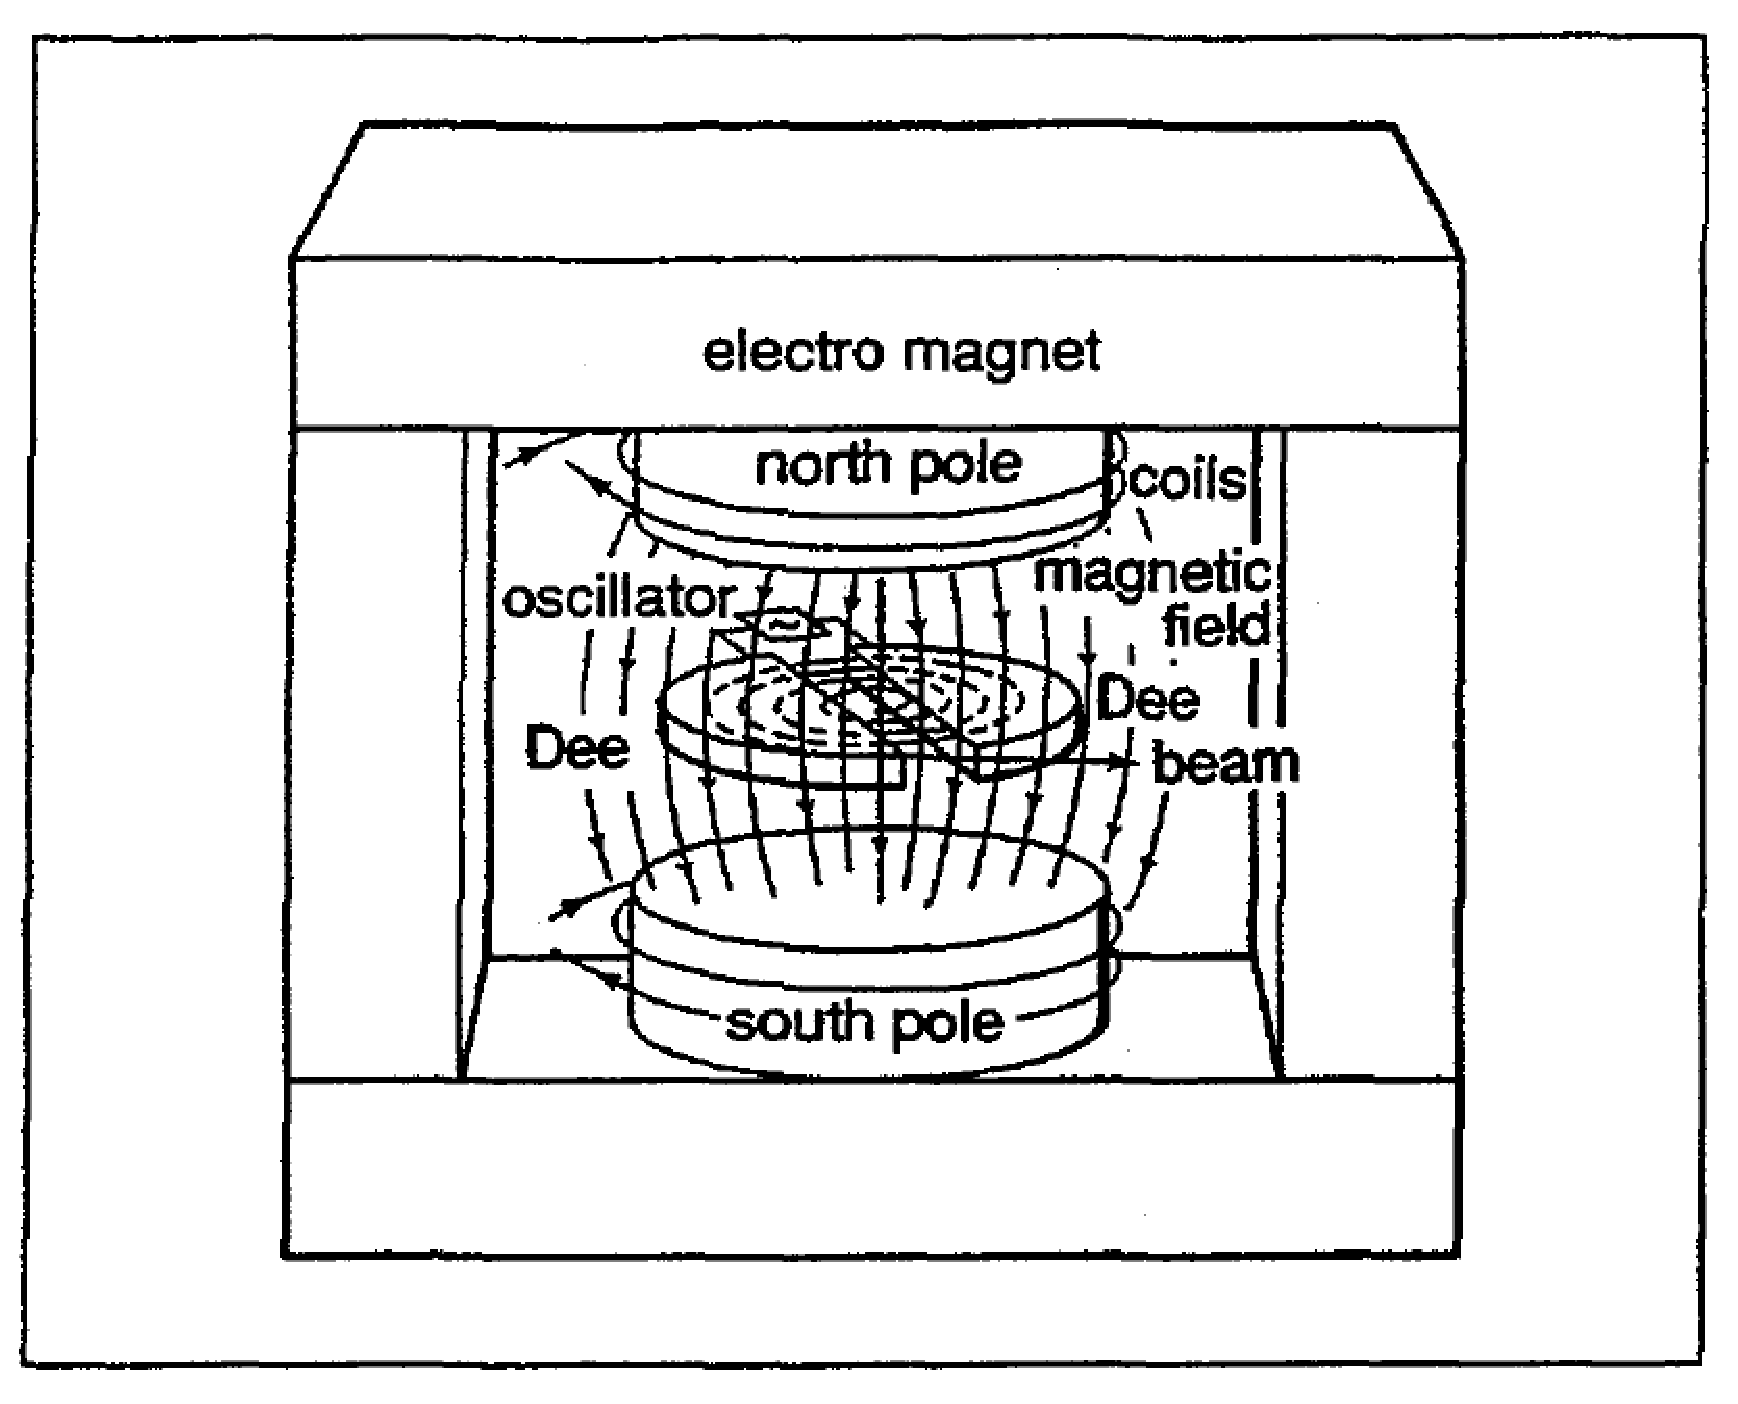
\includegraphics[width=0.45\linewidth]{./figs_cyclo/LBLCycloSketch.eps}
    \caption{A  resonant acceleration device: the cyclotron~[1].} %\cite{CASCycloSketch1994}
    \label{figLBLCycloSketch}
}{
    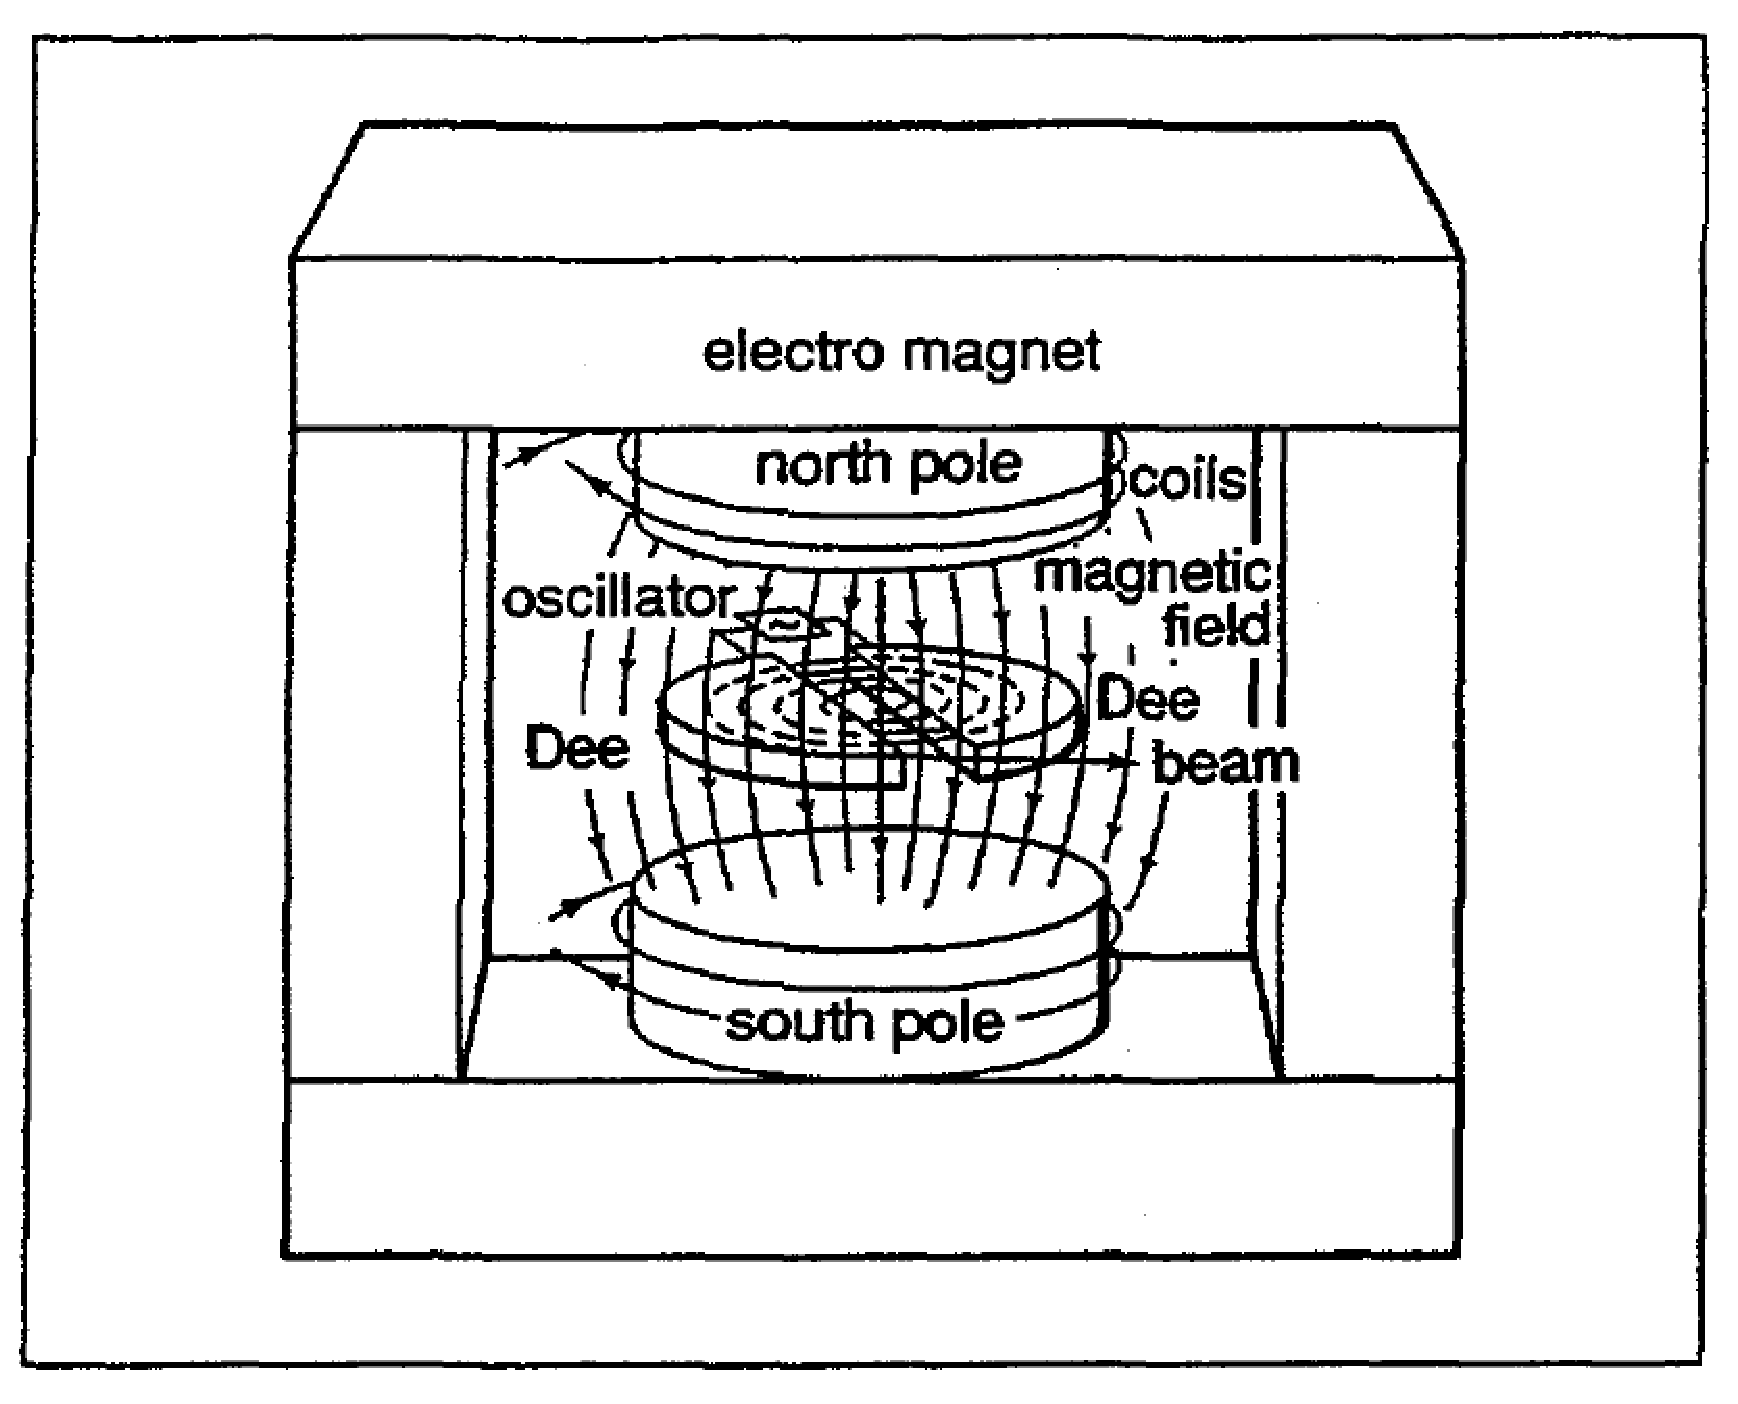
\includegraphics[width=0.45\linewidth]{./figs_cyclo/LBLCycloSketch.eps}
    \caption{The world greatest beam power cyclotron, at PSI.}
    \label{fig1.3}
}
\end{figure}

In a uniform field $B$ a  particle with rest mass $m_0$, 
relativistic mass $m=\gamma m_0$, charge $q$, momentum $p=mv$, undergoes a circular motion
characterized by its radius $R$, with a revolution frequency $f_{\rm rev}$ which depends on the field 
and on the particle charge and mass, but \emph{not} on $R$ neither on the particle velocity. 
Thus repeated acceleration can be provided by a system (the double-gap formed by the double dee in Fig.~\ref{figLBLCycloSketch}) 
with fixed frequency $f_{\rm RF}$ in resonance, at some harmonic integer $h$, 
 with the orbital frequency of the particle. These three quantities satisfy, respectively 
\begin{equation}
\label{EqRCyclo}
 R = p / qB, \hspace{.1\linewidth} 2\pi f_{\rm rev} = v/R = q B / m, \hspace{.1\linewidth} f_{\rm RF} = h f_{\rm rev}
\end{equation}

These expressions hold in both cases of  \emph{classical} cyclotron, which  operates in 
 sub-relativistic regime, relativistic  $\gamma m_0\sim m_0$, 
and  \emph{isochronous} cyclotron which operates in  relativistic regime, $\gamma > 1$.  

From design and beam simulation viewpoints, a cyclotron accelerator is a typical case 
where just putting together drifts and dipoles in a matrix transport 
code won't do. This may at best work for a particular orbit, and will not allow designing the accelerator. 

The common solution os to use a field map, 2- or 3-dimensional. However, mathematical models for the field 
are also a good approach, especially in a preliminary design phase due to the flexibility it brings 
in tayloring the field so to achieve required constrains of orbit excursion limitations, 
focusing, isochronism, etc.

This is the techniques addressed in the exercises. 

\section{Classical cyclotron \label{secCycloClass}}


The classical limit assumes 
 less then $2-3$\% increase in mass, $\gamma\approx 1.02~1.03$.
This means  $\sim$25~MeV for protons, 50~MeV for D and $\alpha$, 
That is enough energy to transmute all nuclei. As a matter of fact, the classical cyclotron allowed discovering 
oodles of nuclear reactions and isotopes. 



\subsection{Closed orbit, time of flight \label{secCycloClassTra}}

\smallskip
\noindent {\small $\bullet$} Exercise~\ref{secCycloClass}-1 

Construct a 45-degree sector mid-plane 2-dimensional field map, with constant vertical field such as to 
achieve a R=0.5~m extraction radius for  10~MeV H- ions (an injector to a higher energy installation, 
typically, with stripping extraction). 
Use a uniform mesh in cylindrical coordinates. 
In a 8-sector configuration (8 times that map, so constituting a complete ring), 
track H- ions on their circular orbit, for a few different momenta ranging from 5~keV to 10~MeV. Plot, 
as a function of momentum, their 
equilibrium orbit radius $R$ and the time of flight $T_{\rm rev}$ on that orbit, 
 from both ray-tracing and  theory on a same graphic. 
Study the effect of the mesh density on the accuracy of trajectory computation. 



\smallskip
\noindent {\small $\bullet$} Exercise~\ref{secCycloClass}-2 
Zgoubi provides analytical models 
 for the magnetic field ${B_y(r,\theta)|_{y=0}}$ in the median plane of a dipole magnet. 
The particular keyword \verb|CYCLOTRON| is an instance.  Use it to repoduce the results above. 
From the two series of results, comment on various pros and cons of the two methods, analytical field models and 
fieldmaps.


\subsection{Acceleration}\label{secCycloAccel}


The RF gap provides a voltage  
\begin{equation}
\label{EqRCyclo}
V_{\rm RF}(t) =\hat V \cos ........... 
\end{equation}
Particles are accelerated as long as they belong in the $[-90,+90]$~degree phase interval, 
the closer to $\phi=90$~deg, the smaller the number of turns 
(the time interval) necessary to reach the extraction radius of the cyclotron.
A deviation of the field B from the isochronous value $2\pi m f_{\rm rev}/q$
will result in a  shift in the arrival phase of the particle at the RF gap amounting to 
\begin{equation}
\label{EqPFPhaseCyclo}
\Delta (\sin \phi) = 2\pi h n \Delta B/B
\end{equation}

 ******* prendre de valeurs R, B, etc. realistes, e.g. in ../biblio/22047216.pdf, 23001796.pdf*******

\smallskip
\noindent {\small $\bullet$} Exercise~\ref{secCycloAccel}-1 
Assume an accelerating double-gap  configuration as in Fig.~\ref{figLBLCycloSketch}. 
What is the minimum number of turns  expected  from 5~keV to 10~MeV~? Track a particle over that range, 
play with the RF phase, conclude on the  expectations. 
In a V(t) diagram, plot  the position  of the particle along the V(t) curve at the 
accelerating gap, for a magnetic field defect 
$\Delta B/B= 10^{-4}$, homogeneous, in the previous sector  map. 




\subsection{Focusing  \label{secCycloFocus}}

Let $B_r$, $B_y$  be the radial and axial components of the magnetic field, respectively, 
$x=r-R$ a small radial displacement with respect to the reference circular orbit,  
$\omega_{\rm rev} = 2\pi f_{\rm rev} $ the angular frequency of the circular motion. 
The radial and axial  strengths experienced by a particle moving in the vicinity of that reference orbit 
write, to the first order in the radial, $x$,  and axial, $y$, coordinates 
\begin{eqnarray}
\label{EqCycloFoc}
F_x = m \ddot x=  -qvB_y + m\frac{v^2}{r} \approx -q v (B_y|_{x=0} + \frac{\partial B_y}{\partial r}x)  + m\frac{v^2}{R}(1-\frac{x}{R}), & \nonumber \\ 
\textrm{~yielding~}  \ddot x + \omega_r^2 x=0 &  \nonumber \\
F_y= m\ddot y =   qvB_r \approx q v \frac{\partial B_r}{\partial y} y = q v \frac{\partial B_y}{\partial r} y, 
 \textrm{~yielding~}    \ddot{y} - \omega_y^2 y= 0  & ~ ~ ~ 
\end{eqnarray}
wherein 
$\omega_r^2 = \omega_{\rm rev}^2(1+\frac{R}{B}\frac{\partial B_y}{\partial r})$,  
$ \omega_y^2 = \omega_{\rm rev}^2 \frac{R}{B} \frac{\partial B_y}{\partial r}$. 
Focusing by a restoring force appears owing to the use of a magnetic field with radial 
index 
\begin{equation}
\label{EqCycloRadialIndex}
k = \frac{R}{B}\frac{\partial B_y}{\partial r}|_{x=0,y=0}
\end{equation}
The two quantities 
\begin{equation}
  \nu_r = \omega_r/\omega_{\rm rev} = \sqrt{1+k},   ~ ~ ~ ~ 
 \nu_y=\omega_y /\omega_{\rm rev}  = \sqrt{-k} 
\end{equation}
are known  respectively as the radial and the axial ``wave number'' of 
the oscilatory motion in the neiboring of the reference circular orbit.
Note that $\nu_r^2 + \nu_y^2=1$.
Vertical motion stability requires $k$ to be negative~:  $B_y$ (respectively, the magnet gap) 
is slowly  decreasing (increasing) with radius, restoring force toward the 
median plane. 
Focussing in both radial and axial motions requires $0 < k <-1$, a conditon known as ``weak focusing''.
 Note that  at low energy  the electric field in the 
region of the accelerating gap also contributes to the focusing, an aspect omitted here. 


\smallskip
\noindent {\small $\bullet$} Exercise~\ref{secCycloFocus}-1
Plot two particle trajectories that demonstrate the value of the radial wave number in the uniform 
field of Sec.~\ref{secCycloClass}. Conclude on orbit and horizontal motion  stability. 
Derive the  vertical  transport matrix from ray-tracing, conclude on the stability of the vertical motion
in a uniform field.


\smallskip
\noindent {\small $\bullet$} Exercise~\ref{secCycloFocus}-2
Back to the field map of exercise~\ref{secCycloClass}-1, or to the analytical model 
of exercise~\ref{secCycloClass}-2: introduce a field index $-1<k<0$. 
Plot the radial and vertical phase space of a 5~MeV ion on a $1\mu$m normalized invariant.  
Compute its radial and axial motion wave numbers, $\nu_r$ and $\nu_y$, 
using two different methods, namely, 1-turn mapping and  Fourrier analysis of multi-turn motion. 
From multiturn tracking, generate the envelope of a 5~MeV beam around the ring cyclotron.  


\smallskip
\noindent {\small $\bullet$} Exercise~\ref{secCycloFocus}-3
Using either the field map or the analytical model devised in the  exercise~\ref{secCycloFocus}-2, 
 plot the energy dependence of the reference orbit radius, $R(E)$. 
Plot  $\nu_r^2 + \nu_y^2$ as a function of radius, compare with the value of the field index. 
On a common graphic, plot the horizontal phase space of the 1, 10, 20, 50~MeV particle motion,
assuming the latter on a $1\mu$m normalized invariant in each case.
Plot the vertical phase space motion for these very energies. 
Plot the components of the field vector experienced by a particle as a function of 
azimutahl angle, over a few turns.


\subsection{Isochronism  \label{secCycloIsochro}}
  

The  condition  for vertical focusing, $-1 < k <0$ 
%  \hspace{2ex} \raisebox{-20mm}[0mm][0mm]{ \includegraphics[width=6cm]{rfCyclo.eps}} \\
spoils the isochronism: the guiding field $B$ and thus $\omega_{\rm rev} = qB/m$ decrease with R (with increasing momentum). 
 As a consequence, the arrival time of a particle at the RF gap (by 
extension the ``RF phase'') is not constant  (ABCDE path)


\smallskip
\noindent {\small $\bullet$} Exercise~\ref{secCycloIsochro}-1


     bunching~: particle beam injected into the cyclotron necessarily gets bunched, at the 
frequency of the RF (the time interval between two bunches is an RF period)




Classical cyclotron $0<n<1$


Isochronous cyclotron, $0<n<1$ cannot be satisfied as $B\propto \gamma$. Introduce Thomas focusing, using sector magnets,
no longer slow r-decrease, weak focusing uniform field.



\subsection{Resonant acceleration}

A tight tuning between particle time-of-flight, which measns in practice the 
field $B$, and the RF frequency is necessary in order to reach the 
resonance condiiton, $f_{\rm RF} = h f_{\rm rev}$.

The accelerating gap in the simulation provide $V_{\rm RF}(t) = \hat V \sin (\omega_{\rm RF} t)$......... 

(i)~Check the evolution of the particle acceleration when 
 getting away from the resonant frequency: \\
- Plot the particle position along the $V_{\rm RF}(t)$ curve in a $V_{\rm RF}(t)$ diagram. \\
- Plot the final phase $\phi_{\rm final}$ as a function of $\Delta B/B$. \\
- Find the tolerable deviation from the isochronous field, 
$\Delta B/B$,  if particles are required to be dispersed in momentum by les 
than $dp/p=10^{-3}$ at the end of the acceleration cycle.




\section{Relativistic cyclotron \label{secCycloRel}}

The bad news with relativistic energies, is, 
the cyclotron resonance $\omega_0 = qB/\gamma m_0$, with $R = \beta c / \omega_0$  yields  
       $$k = \frac{R}{B}\frac{\partial B}{\partial R} = \frac{\beta}{\gamma} 
  \frac{\partial \gamma}{\partial \beta} = \beta^2 \gamma^2 $$
$k$ is positive and increases with energy, 
 the weak focussing condition $-1<k<0$ is not satisfied. 

The time of flight on the equilibrium orbit, momentum $p = qB\rho$ and circumference $\mathcal{C}$, is 
$T =  \mathcal{C}/ \beta c = 2\pi \gamma m_0 / qB$. 
    Isochronism requires $p$-invariant time of flight, $dT/dp=0$. Differentiating the previous expression,
this requirement yields 
$$B = \frac{B_0}{\gamma_0} \gamma$$
with $B_0$ and $\gamma_0$  some refence conditions and time of flight $T_0 = (2\pi m_0/q)(\gamma_0/B_0)$.
In other words, isochronism requires $ B(r) \propto \gamma$, which yields vertical defocusing. 

That was the end of the story in the late 1930s. 
Hans Bethe (1937)~: 
``... it seems useless to build cyclotrons of larger proportions than the  
existing ones... an accelerating chamber of 37 cm radius will  suffice to 
produce deuterons of 11 MeV energy which is the highest possible...''. 
Frank Cole~: ``If you went to graduate school in the 1940s, this inequality ($−1 <
k < 0$) was the end of the discussion of accelerator theory.''

  Until...

\subsection{Thomas focusing}

\begin{itemize}
\item[\bull]  1938, L.H.~Thomas, ``The Paths of Ions in the Cyclotron'', 
introduces the \\
 ``Thomas focusing'', based on separate sector bending, namely,  \\
``edge-focusing'', 
% \hfill  \raisebox{-20mm}[0mm][0mm]{ \includegraphics[width=5cm]{cyclo_Baartman_p6.eps}}
\item[\bull]  1954, Kerst, spiral edges increase vertical focusing further \\
$\nu_z = \sqrt{-k + F^2(1 + 2 \tan^2 \xi)}$, ~ ~ $F=Flutter = \frac{<B^2> - <B>^2}{<B>^2}$
% \hspace{1ex}  \raisebox{-25mm}[0mm][0mm]{ \includegraphics[width=4.8cm]{cyclo_Baartman_p7.eps}}
\item[\bull]  That allowed having $B(r)$ increase in proportion to $\gamma$, so to \\ 
ensure constant RF frequency  ($\omega_0 = qB / \gamma m$), \\
while {\it preserving vertical focusing}.  

\item[\bull]  Modern cyclotrons still rely on these principles


\vspace{0mm}
%\includegraphics[width=10cm]{cycloSpiralOuvert.eps}
%\hspace{0mm}\raisebox{-50mm}[0mm][0mm]{\includegraphics[width=18cm]{cycloMedic-proton_solution_1.eps}}

~

\item[\bull] Cyclotron is limited in energy by its field strength and magnet size. 
\end{itemize}




\subsection*{Exercise}


{
On RF harmonic 1, which RF frequency applied on dees 
is needed to accelerate a proton in a $\sim$uniform, 1~Tesla magnetic field~? 

~

What is the  energy gained by a proton when it reaches $r=0.3\,$m~?
}

~



\subsection*{Exercise}


{
On RF harmonic 1, which RF frequency applied on dees 
is needed to accelerate a proton in a $\sim$uniform, 1~Tesla magnetic field~? 

~

What is the  energy gained by a proton when it reaches $r=0.3\,$m~?
}


~

~

{
Answers~:  

~

1/ $f_{rev.} = e B / 2 \pi m = c^2 B / 2 \pi (mc^2/e) = 9\, 10^{16} \times 1 / 2 \pi 10^9 \approx 15\,$MHz

Two accelerating gaps  at 180~degrees $\Rightarrow  f_{RF} = f_{rev.}$ 

~

~

2/
From $r =\frac{mv}{eB}$ one gets $\frac{1}{2} m v^2 \equiv E  = \frac{1}{2} \frac{(eBr)^2}{m}  = 
\frac{1}{2} \frac{eB^2r^2c^2}{(mc^2/e}  $ hence $\frac{E}{e} (eV) = \frac{1}{2} \frac{B^2r^2c^2}{(mc^2/e)}  $ 

$\frac{E}{e} (eV) = \frac{1}{2} \frac{1^2 (0.3)^2 (3\, 10^8)^2}{10^9} \approx 4.3\, $MeV.  



~
}






\subsection{Orbits}

- find the orbits, energy dependence of radius, time of flight.

Plot these quantities against theoretical expectations


\subsection{Focusing}

Check $Q_x^2 +Q_y^2$. Plot radial dependence of field index n(r), check \verb|0<n(r) <1|.


\subsection{Acceleration}

Introduce a double-Dee simulation. Hint: use CAVITE

Accelerate a complete cycle, on h=1, h=3. In V(t) space, plot V(t) path of reference particle (use PRINT in CAVITE). 






\section{Exercises: hints, help}

\noindent {\small $\bullet$} Exercise~\ref{secCycloAccel}-1 


\section{Bibliography}

Stambach CAS

R Baartman Cyclotrons: Classic to FFAG

